\subsection{Protocol and validation}
Experiments use an Apple M4 Max MacBook with 48\,GiB unified memory, macOS 26.6.2, Apple Clang 21.0.0, Eigen 5.0.1, and an installed BLASFEO archive targeting Apple M1 instructions. The release build uses \texttt{-O3 -DNDEBUG} and double precision. Clarabel 0.11.1 runs through Python 3.13 with NumPy 2.2.6 and SciPy 1.15.3. Solver threads are limited to one. Benchmark processes run sequentially, without concurrent builds or tests. Normal operating-system scheduling remains active, with no core pinning, frequency lock, or temperature control. Consequently these are laptop measurements, not controlled hardware throughput estimates.

The generated suite has 18 deterministic instances: diagonal ellipsoids at three dimensions in native and rotated-cone form, three locally coupled mixed problems, four double-integrator control horizons, and five cone dimensions at fixed two-variable support. The control model has four states, two inputs, 0.2\,s sampling, acceleration norm at most one, and a terminal state ball of radius 0.5. Two continuous plastic-plate problems from CBLIB~\cite{cblib}, \texttt{nql30} and \texttt{nql60}, add 4,501 and 18,001 variables, respectively. They have 3,680 and 14,560 equalities and 900 and 3,600 cones. Both use the general sparse backend.

Each timing batch follows one unrecorded solve. Generated PIQP batches and all Clarabel batches contain 30 solves, while public PIQP batches contain ten. Every solve initializes from scratch. Setup is measured once per instance and backend. Update timings reapply unchanged quadratic bounds and cone offsets. Clarabel timings include the Python call but exclude conversion to the conic model. Table~\ref{tab:time} reports medians, and the archived CSV files retain every observation, residual, status, and the first and third quartiles. Repetitions measure timing dispersion, not additional problem instances.

PIQP requests absolute and relative tolerances of $10^{-8}$. Clarabel requests $10^{-11}$, since looser internal criteria on the plate problems did not meet the same original-coordinate complementarity check. Independent acceptance requires primal feasibility, stationarity, dual-cone membership, and slack consistency within $10^{-7}$, finite variables, and $s^Tz/(1+|f(x)|)\leq10^{-7}$. A rounding allowance applies to nonnegativity of $s^Tz$. Generated PIQP solutions also agree across backends and with available analytic solutions within $10^{-4}$ in maximum norm.

All 54 generated instance/backend combinations and both public solves pass these checks. Clarabel passes its conic-form checks on all 20 instances, with seven \texttt{Solved} and 13 \texttt{AlmostSolved} statuses. However, mapping the lifted duals back to native quadratic multipliers leaves stationarity above $10^{-7}$ on the three native ellipsoid and three mixed instances. Their recovered residuals range from $1.35\times10^{-7}$ to $2.38\times10^{-6}$. These timings therefore do not establish an advantage at matched native-dual accuracy. The supplied conic ellipsoids do pass the conic checks. Across all instances, objective differences remain below $6\times10^{-8}$.

The C++ suite adds 45 tests, including 50 mixed problems with independently constructed KKT points, full Newton-direction comparisons, singular curvature, zero gradients, cone apexes, scale variation, nearly dependent equalities, nonlocal support, and known infeasible models. Tests exercise every sparse elimination mode and the actual BLASFEO multistage factorization. Eigen allocation guards and a C++ allocation counter cover solves and numerical updates. The extension passes AddressSanitizer and UndefinedBehaviorSanitizer checks. Existing QP tests also pass. Infeasible tests check that the solver does not claim a successful solution, rather than demand a certificate that this method does not derive.

\begin{table}[t]
\centering
\caption{Median solve time in milliseconds. Clarabel uses exact cone reformulations for native quadratic rows.}
\label{tab:time}
\small\begin{tabular}{lrrrr}
\toprule
Instance & Dense & Sparse & Multi. & Clarabel\\
\midrule
Quadratic, $n=128$ & 0.630 & 0.050 & 0.255 & 0.216\\
Cone lift, $n=128$ & 1.032 & 8.082 & 1.383 & 0.232\\
Mixed, 64 stages & 4.317 & 0.525 & 0.763 & 1.632\\
Control, $N=80$ & 21.337 & 0.661 & 0.733 & 0.986\\
nql30 & -- & 85.242 & -- & 98.662\\
nql60 & -- & 490.676 & -- & 620.653\\
\bottomrule
\end{tabular}

\end{table}

\begin{figure*}[t]
\centering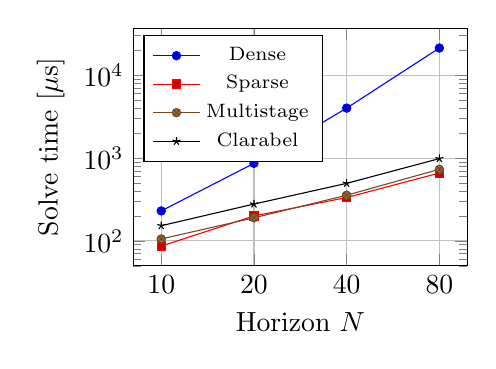
\begin{tikzpicture}
\begin{loglogaxis}[width=.48\textwidth,height=4.6cm,xlabel={Horizon $N$},ylabel={Solve time [$\mu$s]},grid=major,xtick={10,20,40,80},xticklabels={10,20,40,80},legend style={font=\scriptsize},legend pos=north west]
\addplot+[mark size=1.5pt] coordinates {(10,230.354) (20,864.646) (40,4016.31) (80,21337.3)};
\addlegendentry{Dense}
\addplot+[mark size=1.5pt] coordinates {(10,86.625) (20,200.166) (40,334.375) (80,660.604)};
\addlegendentry{Sparse}
\addplot+[mark size=1.5pt] coordinates {(10,105.645) (20,190.041) (40,356.333) (80,732.875)};
\addlegendentry{Multistage}
\addplot+[mark size=1.5pt] coordinates {(10,152.625) (20,278.771) (40,495.646) (80,986.208)};
\addlegendentry{Clarabel}
\end{loglogaxis}
\end{tikzpicture}
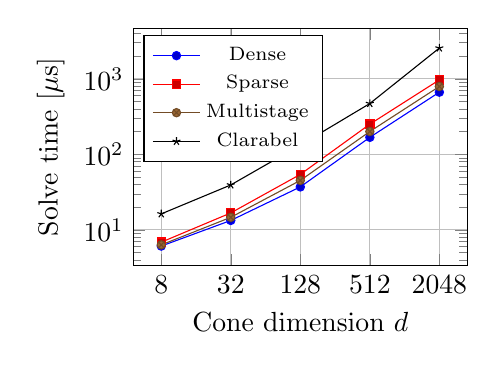
\begin{tikzpicture}
\begin{loglogaxis}[width=.48\textwidth,height=4.6cm,xlabel={Cone dimension $d$},ylabel={Solve time [$\mu$s]},grid=major,xtick={8,32,128,512,2048},xticklabels={8,32,128,512,2048},legend style={font=\scriptsize},legend pos=north west]
\addplot+[mark size=1.5pt] coordinates {(8,6.1045) (32,13.333) (128,37.0625) (512,167.896) (2048,664.98)};
\addlegendentry{Dense}
\addplot+[mark size=1.5pt] coordinates {(8,6.875) (32,16.7705) (128,54.2495) (512,250.75) (2048,967.375)};
\addlegendentry{Sparse}
\addplot+[mark size=1.5pt] coordinates {(8,6.334) (32,14.667) (128,45.1665) (512,200.5) (2048,791.729)};
\addlegendentry{Multistage}
\addplot+[mark size=1.5pt] coordinates {(8,16.291) (32,39.333) (128,132.562) (512,470.604) (2048,2553.94)};
\addlegendentry{Clarabel}
\end{loglogaxis}
\end{tikzpicture}

\caption{Median solve times. Left: control horizon with fixed stage dimensions. Right: cone dimension with fixed two-variable support. The right experiment isolates coordinate work and does not represent a cone with growing variable support.}
\label{fig:scaling}
\end{figure*}

\subsection{Structure and representation}
Figure~\ref{fig:scaling} shows nearly linear control-horizon growth for both sparse and multistage solves. Both take seven iterations at every horizon. The measurements show no consistent multistage speed advantage for these small stage blocks. Dense factorization grows much faster with the horizon. At fixed support, the cone sweep is also approximately linear after the smallest sizes, as expected from the spectral transforms. Iteration counts rise from five to seven over that sweep.

The $n=128$ ellipsoid exposes a different limitation. A native scalar quadratic row retains a small augmented sparse system. Its exact cone lift expands the slack dimension and fills the transformed Jacobian across the entire variable support. The sparse cone solve is much slower than both the native solve and Clarabel on the identical conic representation. Linear-time scaling alone does not remove this fill. A sparse expansion of the cone block, as used by ECOS, is not implemented here. The native quadratic representation avoids that particular expansion cost, but general large-support cones remain a weakness of the whitening adapter.

\subsection{Public problems and profile}
Both plate solutions agree with Clarabel in objective within $7\times10^{-9}$. Their PIQP stationarity residuals are $2.34\times10^{-9}$ and $1.57\times10^{-9}$, and primal violations are below $4\times10^{-14}$. The solve-time interquartile ranges are 84.7--86.2\,ms and 484.9--500.5\,ms. They require 22 and 21 iterations, with 26 and 29 regularization retries and 106 and 95 refinement steps. The retry counts explain why iteration count alone understates their linear-algebra work.

A separate Tracy 0.12.2 capture of 20 \texttt{nql30} solves attributes 38.5\% of exclusive recorded time to sparse numerical factorization and 32.3\% to triangular solves. Newton assembly accounts for 6.9\%. These instrumented timings diagnose cost and are excluded from Table~\ref{tab:time}. Earlier dense cone-scaling matrices were replaced by the spectral operations in Section III-A. This removes cubic cone factorization and quadratic cone storage. Two subsequent experiments used three samples per public problem and variant. Delaying regularization reduction for two iterations after retries, or retaining the raised value as a floor, reduced median solve times by approximately 21--27\%. Neither change was adopted because its difficult-case validation was too narrow.

The transformed Jacobians contain 8,100 and 32,400 stored entries. The permuted upper KKT matrices contain 36,850 and 147,500 entries, while their factors contain 122,642 and 610,684 entries including the diagonal. These symbolic counts include declared numerical zeros but exclude index arrays and other workspaces. Separate process peak resident sizes are 15.8 and 49.5\,MiB. Those observations include input loading, model copies, symbolic counting, and libraries, rather than just solver workspaces. Setup, update, and factorization-plus-assembly timings are retained with the raw data.

The QP regression compares identical box-constrained problems against the original revision, using the same compiler and $10^{-10}$ tolerances. Both versions pass the analytic solution check. The QP implementation is unchanged. Laptop timing variability prevents conclusions about small overhead differences.
